\begin{block}{Conformal Mapping}
  Assuming fore-and-aft symmetry, a conformal map $z=Z (\zeta)$ from the
  conformal domain
  $ \Omega:= \Om^{+} \cup \Om^{-}$
  % $ \Omega:= \left \{ \zeta: \rho < |\zeta| < 1 \right \}$
  to the region
  $\mathcal{D} := \mathcal{D}_{-}\cup\mathcal{D}_{+}$ of the physical
  domain has representation
  \begin{gather}
    \label{eq:conformal}
    Z(\zeta) = \ii a_{0} \left[ \frac{\zeta - \rho}{\zeta + \rho} +
      \alpha(\zeta) - \alpha(\rho^{2}/\zeta) \right]
    \quad\text{with}\quad \alpha(\zeta) = \sum_{k=1}^{\infty} a_{k}
    \zeta^{k} \,,
  \end{gather}
  where $a_{0} \in \RR^{+}$ and $a_{k} \in \RR$ for all $k \in \NN$.

  %%%% Conformal domains %%%%%%%%%%%%%%%%%%%%%%%%%%%%%%%%%%%%%%%%%%%%%%
  \begin{figure}\label{fig:conformal}
    \centering
    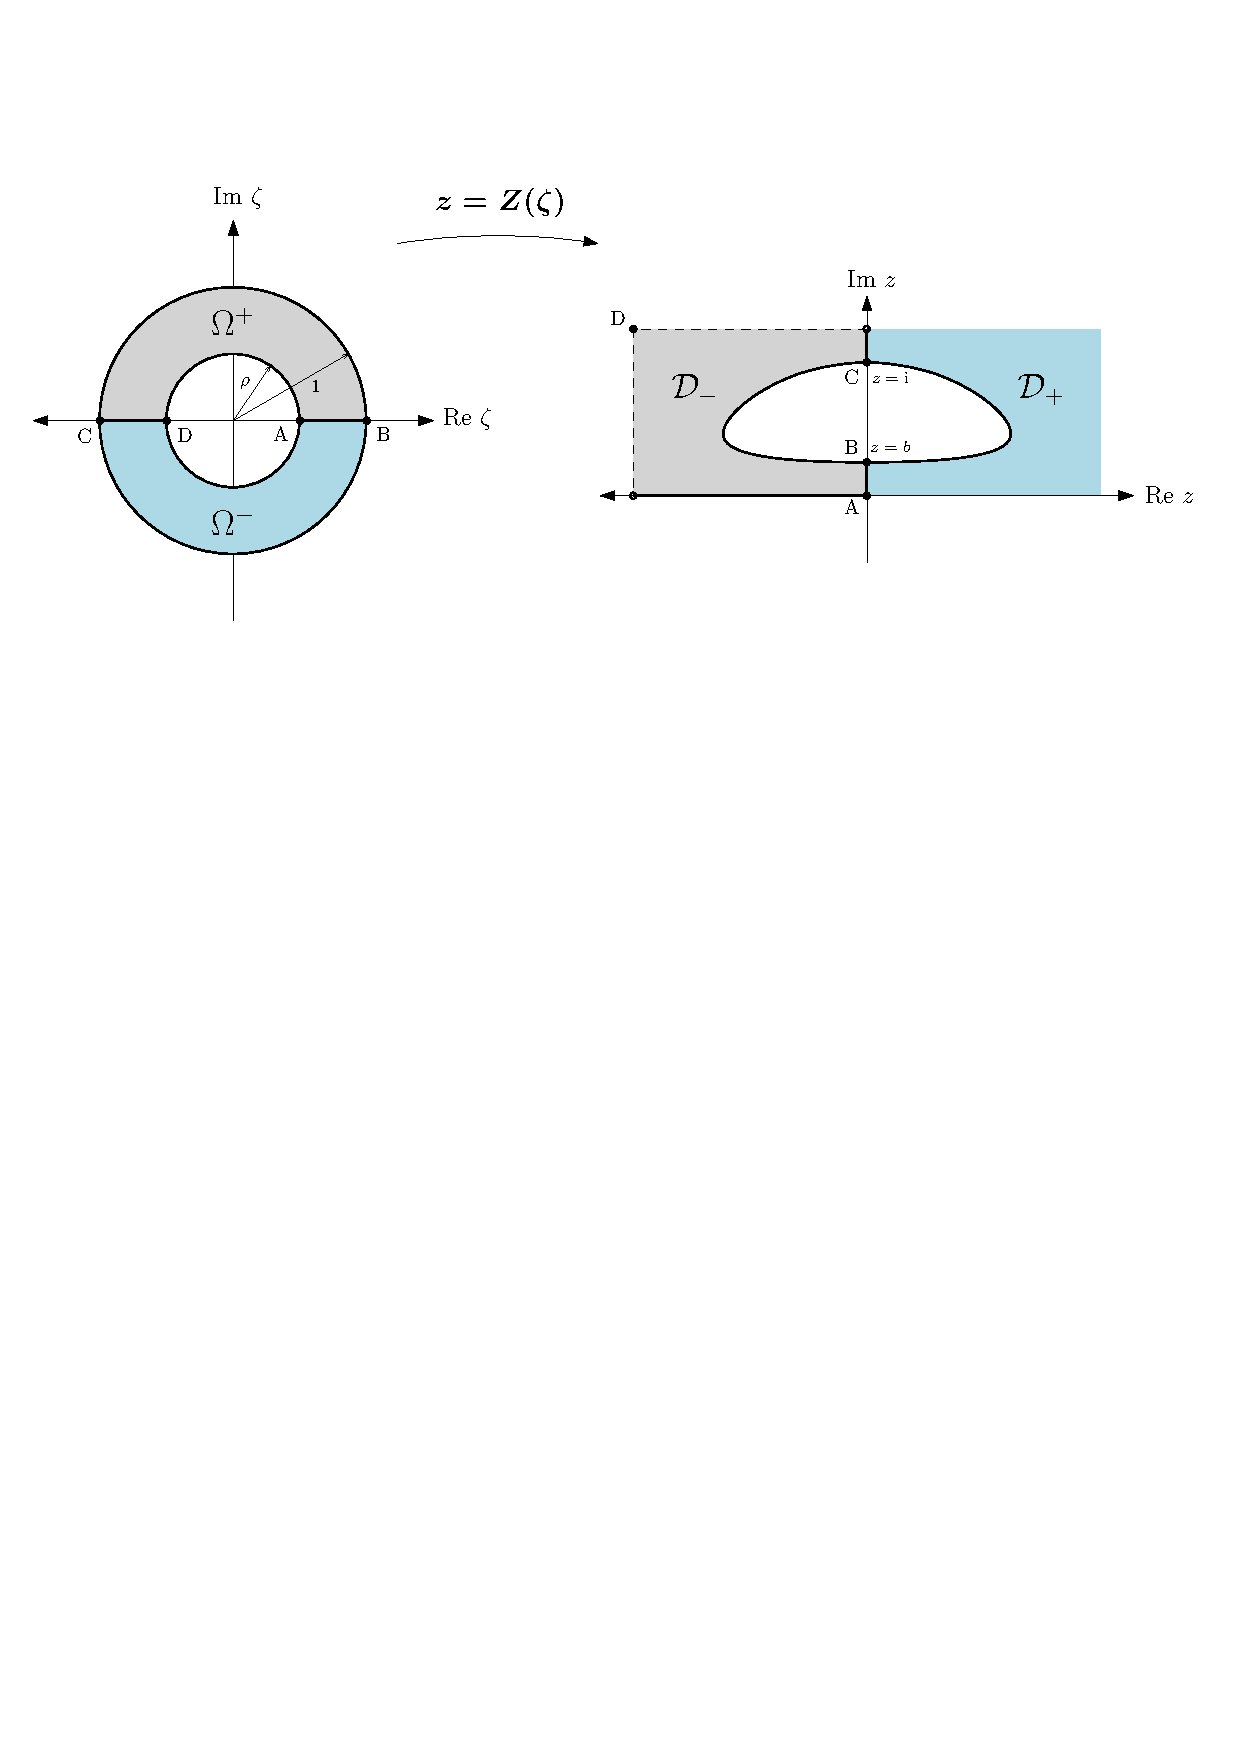
\includegraphics[width=0.95\linewidth]{conformal_continued}
    \caption{Conformal mapping between $\Om$ in the conformal
      $\zeta$-plane and $\cD$ in the physical $z$-plane.}
  \end{figure}

  \textbf{Key observation.}
  \begin{itemize}
  \item $\ii \zeta Z'(\zeta)$ has a double pole at $\zeta = -\rho$
    while $dw/dz - U = O(z^{-2})$ as $z \to \infty$, thus the
    expression
    \begin{equation*}
      \left( \frac{\dd w}{\dd z} - U \right)
      \ii \zeta \frac{\dd Z}{\dd \zeta}
    \end{equation*}
    is singularity-free in $\rho \le \abs{\zeta} \le 1$.
  \item $\ii  \zeta Z'(\zeta) + \cJ(\zeta)$ is singularity-free on
    $\rho \le \abs{\zeta} \le 1$ and is real-valued on
    $\abs{\zeta} = \rho$ and $\abs{\zeta} = 1$ where
    \begin{equation*}
      \mathcal{J} (\zeta) =  2 \zeta \sum_{k=1}^\infty \left[
        \frac{\rho^{2k-1}}{(\zeta+\rho^{2k-1})^2}
        +\frac{\rho^{2k-1}}{(1+\rho^{2k-1} \zeta)^2}
      \right] \,.
    \end{equation*}
  \end{itemize}
\end{block}


\begin{alertblock}{Alternate Formulation: Complex Variable Form}
  Determine a map $Z(\zeta)$ univalent in $\Om$ in the
  form~\eqref{eq:conformal} with $Z'(\zeta)$ existing on $\abs{\zeta}
  = 1$, and a corresponding translation velocity $U$ satisfying
  \begin{equation}\label{eq:complex}
    \Bigl[ U + \cA[Z](\zeta)\Bigr] \ii \zeta Z'(\zeta)
    + U \cJ(\zeta) = \cC[Z] \quad \text{on $\overline{\Om}$,}
  \end{equation}
  where
  \begin{gather}
    \cA[Z](\zeta) = \frac{1}{4\pi} \oint_{\abs{\zeta'}=1}
    \left(
      \frac{ \conj{Z(\zeta) - Z(\zeta')} }
      { Z(\zeta) - Z(\zeta') } +
      \frac{ \conj{Z(\zeta) + Z(\zeta')} }
      { Z(\zeta) + Z(\zeta') }
    \right)
    Z_{\zeta}(\zeta') \; \dd\zeta' \,, \\
    \cC[Z] = \frac{1}{2\pi} \oint_{\abs{\zeta'}=1} \cA[Z](\zeta) Z'(\zeta) \;\dd\zeta \,.
    % \label{eq:J-function}
    % \cJ(\zeta)
    % = 2\zeta \sum_{k=1}^{\infty} \left(
    %   \frac{\rho^{2k-1}}{{\left(\zeta + \rho^{2k-1}\right)}^2}
    %   + \frac{\rho^{2k-1}}{{\left(1 + \rho^{2k-1}\zeta\right)}^2}\
    % \right)\,.
  \end{gather}
\end{alertblock}

\begin{itemize}
\item To deal with highly deformed vortices, \textit{i.e.}, $\rho$ close to 1,
  it is useful to introduce a secondary M\"{o}bius map that maps unit
  circle back to itself:
  \begin{equation}
    \label{eqmobius}
    \zeta = \frac{\eta-\beta}{1-\beta \eta},
    \quad\text{for some suitably choen $\beta \in [0, 1)$.}
  \end{equation}
\item The real coefficients $\left( a_k \right)_{k=1}^\infty $ of the analytic
  function $\alpha$ completely characterize the conformal map $Z$ through the
  representation
  \begin{equation}
    \label{eq1:analytic}
    \alpha \left ( \zeta (\eta) \right ) =
    \sum_{k=1}^\infty a_k \eta^k =
    \sum_{k=1}^\infty a_k \left ( \frac{\zeta+\beta}{1+\beta \zeta} \right )^k
  \end{equation}
  % \item Due to the M\"{o}bius map~\eqref{eqmobius}, the boundary values
  %   of~\eqref{eq:complex} on $\zeta = e^{i\theta}$ can be written in terms of
  %   $\eta = e^{i\nu}$ as follows:
  %   \begin{equation}
  %     \label{eq:1}
  %     z'(\nu) = \theta_{\nu} \frac{C[z] - U j(\nu)}{U + A[z](\nu)}
  %   \end{equation}
  %   where $z(\nu) = Z\left(\zeta(e^{i\nu})\right)$ and $j(\nu) = \cJ\left(\zeta(e^{i\nu})\right)$.
\end{itemize}

%%% Local Variables:
%%% mode: latex
%%% TeX-master: "main"
%%% End:
